\documentclass[11pt]{article}

\usepackage[margin=1.5in]{geometry}
\usepackage{lecnotes}
% \usepackage{mpass}
% \lstset{style=verb,language=mpass}
\input{lmacros}

\newcommand{\course}{15-316: Software Foundations of Security \& Privacy}
\newcommand{\lecturer}{Matt Fredrikson}
\newcommand{\lecdate}{February 24, 2026}
\newcommand{\lecnum}{12}
\newcommand{\lectitle}{Information Flow}
\newcommand{\courseurl}{https://15316-cmu.github.io/2026/}

\begin{document}

\maketitle

\section{Introduction}

In the last lecture we informally introduced a notion of \emph{information flow}
and a type system to ensure \emph{confidentiality}, meaning that high security
data do not flow to low security variables.  The rules are summarized in
\autoref{sec:flowtypes}.  They express an information flow policy as a mapping
$\Sigma$ from variables to security levels, arranged in a semilattice, including
a ghost variable $\mi{pc}$ to track \emph{implicit flows} due to conditional
tests.  We often worked with the two element lattice with levels $\ms{H}$ (for
\emph{high}) and $\ms{L}$ (for \emph{low}) with $\ms{L} \sqsubset \ms{H}$.

We assumed that an attacker can see the program and control or see the values of
all low security variables before and after computation.  We also assumed the
attacker can not observe nontermination (including abort after a failed test);
some of the rules would have to be changed to account for that and still capture
confidentiality.

These rules are \emph{syntactic} and it is straightforward to see that they
define an algorithm for deriving that a program $\alpha$ is secure with respect
to a security policy $\Sigma$ that assigns security levels.

What was missing was a formal \emph{semantic} definition of information flow
security and a proof that the rules are \emph{sound} with respect to this
definition.  That's the goal of today's lecture.  The material is adapted mostly
from \citet{Volpano96jcs}.

\section{Noninterference}

We have already seen that information flow is not a property of a single trace.
Simplifying the example further, consider the security policy
$\Sigma_0 = (x : \ms{H}, y : \ms{L})$, the initial state $x = 0, y = 0$
and the programs
\[
  \begin{array}{c@{\hspace{5em}}c}
    y := x + 1 & y := 1
  \end{array}
\]
The traces are the same, consisting of just one transition
\[
  (x = 0, y = 0) \Rightarrow (x = 0, y = 1)
\]
The program on the left violates our policy, flowing information from $x$ to $y$
to the extent an attacker can fully recover the initial value of $x$ from the
value of $y$ in the final state.  The program on the right permits no such
inference.

If we have just two security levels ($\ms{L}$ and $\ms{H}$) we'd like to
formalize our attacker model using a notion of \emph{observation}.  We consider
the program secure if two initial states are equivalent as far as the attacker
can see, then the final states must also be equivalent as far as the attacker
can see.  If that were not the case, the attacker may be able to make an
inference about the secret (hidden) part of the initial state.

We define when two states $\omega_1$ and $\omega_2$ are \emph{observationally
  equivalent at level $\ms{L}$ with respect to security policy $\Sigma$},
written as $\Sigma \vdash \omega_1 \approx_{\ms{L}} \omega_2$:
\begin{quote}
  We define $\Sigma \vdash \omega_1 \approx_{\ms{L}} \omega_2$
  iff $\omega_1(x) = \omega_2(x)$ for all $x$ such that $\Sigma(x) = \ms{L}$.
\end{quote}
In our tiny example (with $\Sigma_0 = (x : \ms{H}, y : \ms{L})$), we have
(among others):
\[
  \begin{array}{lcl}
    \Sigma_0 \vdash (x = 0, y = 0) & \approx_{\ms{L}} & (x = 0, y = 0) \\
    \Sigma_0 \vdash (x = 0, y = 0) & \approx_{\ms{L}} & (x = 1, y = 0) \\
    \Sigma_0 \vdash (x = 0, y = 1) & \not\approx_{\ms{L}} & (x = 0, y = 2) \\
    \Sigma_0 \vdash (x = 0, y = 1) & \not\approx_{\ms{L}} & (x = 1, y = 2) 
  \end{array}
\]
Next we define that a program $\alpha$ satisfies \emph{noninterference} if
values of high security variables do not affect the outcome as it may be
observed at low security.  We describe outcomes using the relational program
semantics $\omega \lbb \alpha \rbb \nu$ introduced in
\href{\courseurl/lectures/02-semantics.pdf}{Lecture 2}.
\begin{quote}
  We define that program $\alpha$ satisfies \emph{noninterference with respect to
    policy $\Sigma$}\newline iff for all $\omega_1$, $\omega_2$, $\nu_1$, and $\nu_2$,\newline
  $\Sigma \vdash \omega_1 \approx_{\ms{L}} \omega_2$,
  $\omega_1 \lbb \alpha \rbb \nu_1$, and $\omega_2 \lbb \alpha \rbb \nu_2$
  implies $\Sigma \vdash \nu_1 \approx_{\ms{L}} \nu_2$.
\end{quote}
This definition relies on the fact that our language is deterministic: each
initial state has at most one final state.  In a nondeterministic language we
would need to compare sets of possible low-observable outcomes, not just a
single run from each initial state.  Noninterference also does not talk about
the case where there is no final state, which is why this condition is called
\emph{termination-insensitive noninterference}.

Let's apply it to our example.  We want to show that the first program,
$y := x + 1$ does \textbf{not} satisfy noninterference.  That is, we need
to find two states, indistinguishable at level $\ms{L}$, that have
distinguishable outcomes.  So we pick
\[
  \omega_1 = (x = 0, y = 0)\ \mbox{and}\ \omega_2 = (x = 1, y = 0)
\]
As we already determined, we have $\Sigma_0 \vdash \omega_1 \approx_{\ms{L}} \omega_2$.
We further have
\[
  \begin{array}{lcl}
    \omega_1 \lbb y := x+1 \rbb \nu_1
    & \mbox{where} & \nu_1(x) = 0,\ \nu_1(y) = 1 \\
    \omega_2 \lbb y := x+1 \rbb \nu_2
    & \mbox{where} & \nu_2(x) = 1,\ \nu_2(y) = 2
  \end{array}
\]
and $\Sigma_0 \vdash \nu_1 \not\approx_{\ms{L}} \nu_2$ because
the low-observable outcomes for $y$ are different.

On the other hand, for any two (relevant) states that are low-observably
equivalent
\[
  \omega_1 = (x = a, y = b)\ \mbox{and}\ \omega_2 = (x = a', y = b)
\]
we have
\[
  \begin{array}{lcl}
    \omega_1 \lbb y := 1 \rbb \nu_1
    & \mbox{where} & \nu_1(x) = a,\ \nu_1(y) = 1 \\
    \omega_2 \lbb y := 1 \rbb \nu_2
    & \mbox{where} & \nu_2(x) = a',\ \nu_2(y) = 1
  \end{array}
\]
and
\[
  \Sigma_0 \vdash \nu_1 \approx_{\ms{L}} \nu_2
\]
So the program $y := 1$ \emph{does} satisfy noninterference.

By analogous reasoning,\footnote{we did not discover this in lecture} the
program $y := (x-x) + 1$ also satisfies noninterference, even though our type
system would reject it.  This is the first example showing the
\emph{incompleteness} of the proposed type system with respect to information
flow.  Static type systems often have to make \emph{sound} (and decidable)
approximations to some underlying semantic property (which is often
undecidable).

Before we move on, we generalize the noninterference property to an arbitrary
semilattice of security levels.  First, observations are restricted
to all levels \emph{below} a given security level $\ell$:
\begin{quote}
  We define $\Sigma \vdash \omega_1 \approx_\ell \omega_2$
  iff $\omega_1(x) = \omega_2(x)$ for all $x$ such that $\Sigma(x) \sqsubseteq \ell$.
\end{quote}
From this, semantic security with respect to an information flow policy $\Sigma$
generalizes the previous definition in a straightforward way.
\begin{quote}
  We define $\Sigma \models \alpha\; \ms{secure}$
  iff for all $\omega_1$, $\omega_2$, $\nu_1$, $\nu_2$, and $\ell$ \newline
  $\Sigma \vdash \omega_1 \approx_\ell \omega_2$,
  $\omega_1 \lbb \alpha \rbb \nu_1$, and $\omega_2 \lbb \alpha \rbb \nu_2$
  implies $\Sigma \vdash \nu_1 \approx_\ell \nu_2$.
\end{quote}

The soundness property now states:
\begin{quote}
  If $\Sigma \vdash \alpha\; \ms{secure}$ then $\Sigma \models \alpha\; \ms{secure}$
\end{quote}
The completeness property would go in the other direction, but it does not hold
as the small example $y := (x-x) + 1$ from above shows.  We will have another
example at the end of this lecture.

\section{Read Levels of Expressions and Formulas}

We will need some properties of expressions and formulas.  Usually, we would
wait until we find we need them in proving the main theorem (in this case,
soundness), but we show them first because they bring up the important proof
technique of \emph{rule induction}.

The first is that expressions read only below their security level.  The proof
is by rule induction, which means we have to show that all rules preserve the
stated property: if we assume it for all premises then it must hold for the
conclusion.  We have already implicitly used it when proving soundness of
inference rules (for example, for sequent calculus for propositional logic and
dynamic logic).  The reason that every sequent we can derive is valid is that
each inference rule preserves validity.

\begin{lemma}[Expression Read Level]
  \label{lm:exp-read}
  If $\Sigma \vdash e : \ell$ then for every $x \in \ms{use}\; e$,
  $\Sigma(x) \sqsubseteq \ell$.
\end{lemma}
\begin{proof}
  By rule induction on the derivation of $\Sigma \vdash e : \ell$.  We
  consider each case in turn.
  \begin{description}
  \item[Case:]
    \[
      \infer[\ms{const}F]
      {\Sigma \vdash c : \bot}
      {}
    \]
    Then $\ms{use}\; c = \{\,\}$ and the property is vacuously true.
  \item[Case:]
    \[
      \infer[\ms{var}F]
      {\Sigma \vdash x : \ell}
      {\Sigma(x) = \ell}
    \]
    Then $\ms{use}\; x = \{x\}$ and $\Sigma(x) = \ell$, so our property is
    satisfied by reflexivity ($\Sigma(x) = \ell \sqsubseteq \ell$).
  \item[Case:]
    \[
      \infer[\ms{+}F]
      {\Sigma \vdash e_1 + e_2 : \ell_1 \sqcup \ell_2}
      {\Sigma \vdash e_1 : \ell_1
        & \Sigma \vdash e_2 : \ell_2}
    \]
    We have
    \begin{tabbing}
      for all $x \in \ms{use}\; e_1$, $\Sigma(x) \sqsubseteq \ell_1$
      \` (by ind.\ hyp.) \\
      for all $x \in \ms{use}\; e_2$, $\Sigma(x) \sqsubseteq \ell_2$
      \` (by ind.\ hyp.) \\
      $x \in \ms{use}\; (e_1 + e_2)$ \` (assumption) \\
      $x \in \ms{use}\; e_1$ or $x \in \ms{use}\; e_2$
      \` (by defn.\ of $\ms{use}$) \\
      $\Sigma(x) \sqsubseteq \ell_1$ or $\Sigma(x) \sqsubseteq \ell_2$
      \` (from uses of the ind.\ hyp.) \\
      $\Sigma(x) \sqsubseteq \ell_1 \sqcup \ell_2$
      \` (by property of $\sqcup$)
    \end{tabbing}
  \end{description}
\end{proof}

The next lemma has the same kind of proof, so we won't bother writing
it out.

\begin{lemma}[Formula Read Level]
  \label{lm:form-read}
  If $\Sigma \vdash P : \ell$ then for every $x \in \ms{use}\; P$,
  $\Sigma(x) \sqsubseteq \ell$.
\end{lemma}
\begin{proof}
  By rule induction, as in the proof of \autoref{lm:exp-read}.
\end{proof}

\section{Soundness of the Information Flow Type System}

We want to prove that $\Sigma \vdash \alpha\; \ms{secure}$ then
$\Sigma \models \alpha\; \ms{secure}$.  As we might expect from the proofs in
the preceding section, this should follow by rule induction on
$\Sigma \vdash \alpha\; \ms{secure}$.

Before doing this more rigorously, we examine assignment, one of the
base cases.

\begin{theorem}[Soundness of Information Flow Types]
  If $\Sigma \vdash \alpha\; \ms{secure}$
  then $\Sigma \models \alpha\; \ms{secure}$
\end{theorem}
\begin{proof}
  By rule induction on $\Sigma \vdash \alpha\; \ms{secure}$.  We'll need one
  more lemma, which we state and prove later for pedagogical purposes.
\begin{description}
\item[Case:]
  \[
    \infer[\mb{:=}F]
    {\Sigma \vdash x := e\; \ms{secure}}
    {\Sigma \vdash e : \ell
      & \ell' = \Sigma(\mi{pc}) \sqcup \ell
      & \ell' \sqsubseteq \Sigma(x)}
  \]
  We have to show that $\Sigma \models x := e\; \ms{secure}$.
  We have the following setup:
  \begin{tabbing}
    $\Sigma \vdash \omega_1 \approx_k \omega_2$ \` (assumption) \\
    $\omega_1 \lbb x := e \rbb \nu_1$ \` (assumption) \\
    $\omega_2 \lbb x := e \rbb \nu_2$ \` (assumption) \\
    $\ldots$ \\
    $\Sigma \vdash \nu_1 \approx_k \nu_2$ \` (to show)
  \end{tabbing}
  By the definition of $\lbb{-}\rbb$ for assignments we obtain
  \begin{tabbing}
    $\nu_1 = \omega_1[x \mapsto c_1]$ for $c_1 = \omega_1 \lbb e \rbb$
    \` (by defn.\ of $\lbb{-}\rbb$) \\
    $\nu_2 = \omega_2[x \mapsto c_2]$ for $c_2 = \omega_2 \lbb e \rbb$
    \` (by defn.\ of $\lbb{-}\rbb$) \\
  \end{tabbing}
  
  Let's also depict what we know about the security levels.
  \[
    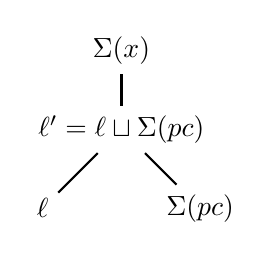
\begin{tikzpicture}
      \node (l) at (0,0) {$\ell$};
      \node (pc) at (2,0) {$\Sigma(\mi{pc})$};
      \node (l') at (1,1) {$\ell' = \ell \sqcup \Sigma(\mi{pc})$};
      \node (x) at (1,2) {$\Sigma(x)$};
      \draw[thick] (l) -- (l');
      \draw[thick] (pc) -- (l');
      \draw[thick] (l') -- (x);
    \end{tikzpicture}
  \]
  At this point we distinguish two cases: $\Sigma(x) \sqsubseteq k$
  and $\Sigma(x) \not\sqsubseteq k$.

  If $\Sigma(x) \sqsubseteq k$ then also $\ell \sqsubseteq k$ by transitivity.
  Since $\Sigma \vdash e : \ell$ and $\Sigma \vdash \omega_1 \approx_k \omega_2$
  we conclude by \autoref{lm:exp-read} that $c_1 = c_2$ and so
  $\Sigma \vdash \omega_1[x \mapsto c_1] \approx_k \omega_2[x \mapsto c_2]$.

  If $\Sigma(x) \not\sqsubseteq k$ then
  $\Sigma \vdash \omega_1[x \mapsto c_1] \approx_k \omega_2[x \mapsto c_2]$
  because $x$ is not observable at level $k$ and
  $\Sigma \vdash \omega_1 \approx_k \omega_2$.

\item[Case:]
  \[
    \infer[\mb{\semi}F]
    {\Sigma \vdash \alpha \semi \beta\; \ms{secure}}
    {\Sigma \vdash \alpha\; \ms{secure}
      & \Sigma \vdash \beta\; \ms{secure}}
  \]
  We set up this case:
  \begin{tabbing}
    $\Sigma \vdash \omega_1 \approx_k \omega_2$ \` (assumption) \\
    $\omega_1 \lbb \alpha \semi \beta \rbb \nu_1$ \` (assumption) \\
    $\omega_2 \lbb \alpha \semi \beta \rbb \nu_2$ \` (assumption) \\
    $\ldots$ \\
    $\Sigma \vdash \nu_1 \approx_k \nu_2$ \` (to show)
  \end{tabbing}
  We can reason with the definition of $\lbb{-}\rbb$.
  \begin{tabbing}
    $\omega_1 \lbb \alpha \rbb \mu_1$ 
    and $\mu_1 \lbb \beta \rbb \nu_1$ for some $\mu_1$
    \` (by defn.\ of $\lbb{-}\rbb$) \\
    $\omega_2 \lbb \alpha \rbb \mu_2$ 
    and $\mu_2 \lbb \beta \rbb \nu_2$ for some $\mu_2$
    \` (by defn.\ of $\lbb{-}\rbb$)
  \end{tabbing}
  Next, by induction hypothesis $\Sigma \models \alpha\; \ms{secure}$
  and together with the assumption about $\Sigma \vdash \omega_1 \approx_k \omega_2$
  we get
  \begin{tabbing}
    $\Sigma \vdash \mu_1 \approx_k \mu_2$ \` (by ind.\ hyp.\ on first premise)
  \end{tabbing}
  This is the fact we need to apply the induction hypothesis on the security
  of $\beta$, because $\beta$ is executed in states $\mu_1$ and $\mu_2$.
  \begin{tabbing}
    $\Sigma \vdash \nu_1 \approx_k \nu_2$ \` (by ind.\ hyp.\ on second premise)
  \end{tabbing}
  Fortunately, this is just what we needed to show.

\item[Case:]
  \[
    \infer[\mb{if}F]
    {\Sigma \vdash \mb{if}\; P\; \mb{then}\; \alpha\; \mb{else}\; \beta\; \ms{secure}}
    {\Sigma \vdash P : \ell
      & \ell' = \Sigma(\mi{pc}) \sqcup \ell
      & \Sigma' = \Sigma[\mi{pc} \mapsto \ell']
      & \Sigma' \vdash \alpha\; \ms{secure}
      & \Sigma' \vdash \beta\; \ms{secure}}
  \]
  This is the most difficult case since it involves implicit flows and therefore
  the ghost variable $\mi{pc}$.  It will require a lemma.  But first we set up:
  \begin{tabbing}
    $\Sigma \vdash \omega_1 \approx_k \omega_2$ \` (assumption) \\
    $\omega_1 \lbb \mb{if}\; P\; \mb{then}\; \alpha\; \mb{else}\; \beta \rbb \nu_1$ \` (assumption) \\
    $\omega_2 \lbb \mb{if}\; P\; \mb{then}\; \alpha\; \mb{else}\; \beta \rbb \nu_2$ \` (assumption) \\
    $\ldots$ \\
    $\Sigma \vdash \nu_1 \approx_k \nu_2$ \` (to show)
  \end{tabbing}
  Here is what we know about the security levels in the rule.
  \[
    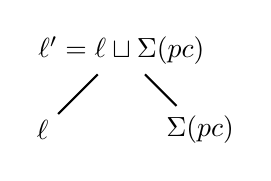
\begin{tikzpicture}
      \node (l) at (0,0) {$\ell$};
      \node (pc) at (2,0) {$\Sigma(\mi{pc})$};
      \node (l') at (1,1) {$\ell' = \ell \sqcup \Sigma(\mi{pc})$};
      % \node (x) at (1,2) {$\Sigma(x)$};
      \draw[thick] (l) -- (l');
      \draw[thick] (pc) -- (l');
      % \draw[thick] (l') -- (x);
    \end{tikzpicture}
  \]
  Again, we distinguish two cases: $\ell' \sqsubseteq k$ and $\ell' \not\sqsubseteq k$.

  If $\ell' \sqsubseteq k$ then also $\ell \sqsubseteq k$ and
  $\omega_1 \models P$ iff $\omega_2 \models P$ by \autoref{lm:form-read}.  If
  both satisfy $P$, we can apply the induction hypothesis to the first premise
  and the executions $\omega_1 \lbb \alpha \rbb \nu_1$ and
  $\omega_2 \lbb \alpha \rbb \nu_2$.  If both do not satisfy $P$, the same
  argument applies to $\beta$.

  If $\ell' \not\sqsubseteq k$ then $\omega_1 \models P$ and $\omega_2 \models P$
  might differ and the different branches might be taken.  In that case we need
  to prove that, nevertheless, whenever $\omega_1 \lbb \alpha \rbb \nu_1$ and
  $\omega_2 \lbb \beta \rbb \nu_2$ we still have
  $\Sigma \vdash \nu_1 \approx_k \nu_2$.

  At this point we can only conclude that because the security level of the
  $\mi{pc}$ is increased to $\ell'$.  The salient property is that if
  $\Sigma' \vdash \alpha\; \ms{secure}$ and $\Sigma'(\mi{pc}) = \ell'$, then
  $\alpha$ \emph{will only write to variables with security level above
    $\ell'$}.  And the same for $\beta$.  (These are instances of
  \autoref{lm:confinement}.)  Fortunately, $\ell' \not\sqsubseteq k$, so none of
  the writes of $\alpha$ and $\beta$ will be observable at level $k$ or below
  and $\Sigma \vdash \nu_1 \approx_k \nu_2$.

\item[Case:]
  \[
    \infer[\mb{test}F]
    {\Sigma \vdash \mb{test}\; P\; \ms{secure}}
    {\mathstrut}
  \]
  We set up:
  \begin{tabbing}
    $\Sigma \vdash \omega_1 \approx_k \omega_2$ \` (assumption) \\
    $\omega_1 \lbb \mb{test}\; P \rbb \nu_1$ \` (assumption) \\
    $\omega_2 \lbb \mb{test}\; P \rbb \nu_2$ \` (assumption) \\
    $\ldots$ \\
    $\Sigma \vdash \nu_1 \approx_k \nu_2$ \` (to show)
  \end{tabbing}
  By definition of $\lbb{-}\rbb$ for tests we know that
  $\omega_1 \models P$, $\omega_2 \models P$, $\nu_1 = \omega_1$, and
  $\nu_2 = \omega_2$.  So the desired conclusion follows immediately from the
  strong assumption that a poststate actually exists.

\item[Case:]
  \[
    \infer[\mb{while}F]
    {\Sigma \vdash \mb{while}\; P\; \alpha\; \ms{secure}}
    {\Sigma \vdash P : \ell
      & \ell' = \Sigma(\mi{pc}) \sqcup \ell
      & \Sigma' = \Sigma[\mi{pc} \mapsto \ell']
      & \Sigma' \vdash \alpha\; \ms{secure}}
  \]
  This case is similar to the case for conditional and we leave it to the
  reader.  Writing it out is a good test of your understanding!
\end{description}
\end{proof}

What remains is the \emph{confinement lemma} relating the security level of the
ghost variable $\mi{pc}$ to the writing behavior of the program.  We define
$\ms{maydef}\; \alpha$ as the set of variables that a program may assign a value
to---just all the left-hand sides of assignments in $\alpha$.  This can include
more variables than the set $\ms{def}\; \alpha$ which includes only those
variables that $\alpha$ must write to.

\begin{lemma}[Confinement]
  \label{lm:confinement}
  If $\Sigma \vdash \alpha\; \ms{secure}$ then for every
  $x \in \ms{maydef}\; \alpha$, $\Sigma(\mi{pc}) \sqsubseteq \Sigma(x)$.
\end{lemma}
\begin{proof}
  By rule induction on $\Sigma \vdash \alpha\; \ms{secure}$.  The key
  observation is that for an assignment $x := e$ the rules require that
  $\Sigma(\mi{pc}) \sqsubseteq \Sigma(x)$ and that the other rules only maintain
  or raise the level.  We elide the case-by-case detail.
\end{proof}

We conclude the lecture with another example that, according to the definition,
satisfies noninterference but we cannot derive that within the type system.
\[
  \mb{if}\; x = 0\; \mb{then}\; y := 1\; \mb{else}\; y := 1
\]
In the type system this fails with $\Sigma_0 = (x : \ms{H}, y : \ms{L})$ because
the assignments in the two branches are to low-security variables.  It is
nevertheless secure because the two values of $y$ are the same, so the
observable outcomes at low level are equal.

\section{Summary: Information Flow Type System}
\label{sec:flowtypes}

\begin{figure}[ht]
  \begin{rules}
    \hspace*{-1em}\fbox{$\Sigma \vdash e : \ell$}\hfill
    \\[1ex]
    \infer[\ms{var}F]
    {\Sigma \vdash x : \ell}
    {\Sigma(x) = \ell}
    \hspace{1em}
    \infer[\ms{const}F]
    {\Sigma \vdash c : \bot}
    {}
    \hspace{1em}
    \infer[\ms{+}F]
    {\Sigma \vdash e_1 + e_2 : \ell}
    {\Sigma \vdash e_1 : \ell_1
      & \Sigma \vdash e_2 : \ell_2
      & \ell = \ell_1 \sqcup \ell_2}
    \\[1em]%\hline
    \hspace*{-1em}\fbox{$\Sigma \vdash P : \ell$}\hfill
    \\[1ex]
    \infer[{\leq}F]
    {\Sigma \vdash e_1 \leq e_2 : \ell_1 \sqcup \ell_2}
    {\Sigma \vdash e_1 : \ell_1
      & \Sigma \vdash e_2 : \ell_2}
    \hspace{2em}
    \infer[{\top}F]
    {\Sigma \vdash \top : \bot}
    {}
    \hspace{2em}
    \infer[{\land}F]
    {\Sigma \vdash P \land Q : \ell_1 \sqcup \ell_2}
    {\Sigma \vdash P : \ell_1
      & \Sigma \vdash Q : \ell_2}
    \\[1em]%\hline
    \hspace*{-1em}\fbox{$\Sigma \vdash \alpha\; \ms{secure}$}\hfill
    \\[1ex]
    \infer[\mb{:=}F]
    {\Sigma \vdash x := e\; \ms{secure}}
    {\Sigma \vdash e : \ell
      & \ell' = \Sigma(\mi{pc}) \sqcup \ell
      & \ell' \sqsubseteq \Sigma(x)}
    \hspace{3em}
    \infer[\mb{\semi}F]
    {\Sigma \vdash \alpha \semi \beta\; \ms{secure}}
    {\Sigma \vdash \alpha\; \ms{secure}
      & \Sigma \vdash \beta\; \ms{secure}}
    \\[1em]
    \infer[\mb{if}F]
    {\Sigma \vdash \mb{if}\; P\; \mb{then}\; \alpha\; \mb{else}\; \beta\; \ms{secure}}
    {\Sigma \vdash P : \ell
      & \ell' = \Sigma(\mi{pc}) \sqcup \ell
      & \Sigma' = \Sigma[\mi{pc} \mapsto \ell']
      & \Sigma' \vdash \alpha\; \ms{secure}
      & \Sigma' \vdash \beta\; \ms{secure}}
    \\[1em]
    \infer[\mb{while}F]
    {\Sigma \vdash \mb{while}\; P\; \alpha\; \ms{secure}}
    {\Sigma \vdash P : \ell
      & \ell' = \Sigma(\mi{pc}) \sqcup \ell
      & \Sigma' = \Sigma[\mi{pc} \mapsto \ell']
      & \Sigma' \vdash \alpha\; \ms{secure}}
    \\[1em]
    \infer[\mb{test}F]
    {\Sigma \vdash \mb{test}\; P\; \ms{secure}}
    {\mathstrut}
  \end{rules}
  \caption{Information Flow Type System\newline
  Termination insensitive, ensuring confidentiality}
  \label{fig:flowtypes}
\end{figure}

\bibliographystyle{plainnat}
\bibliography{bibliography}

\end{document}
